\documentclass{adonis}
\usepackage{hyperref}
\usepackage{tabularx}
\usepackage{xurl}
\usepackage{graphicx}
\usepackage{float}
\usepackage{caption}
\usepackage{pgfplots}
\usepackage{pgf-pie}
\usepackage{tikz}
\usepackage{geometry}
\usepackage{booktabs}
\usepackage{threeparttable}
\usepackage{array}
\geometry{margin=1in}
\usetikzlibrary{positioning, calc}
\pgfplotsset{compat=1.18}
\usepackage[natbib, style=apa]{biblatex}
\addbibresource{bibliography.bib} 
\usepackage{longtable}
\usepackage{booktabs}

% main details
\title{Is the Grass Really Greener on Greenland’s Side? Strategic Trade Diversion and American Geoeconomic Ambitions}
\subtitle{The Role, Or Lack Thereof, of Classical Trade Theory in Geopolitical Strategy}
\author{Erika Salvador \textsuperscript{1}}

% secondary details
\affiliation{\textsuperscript{1} Department of Economics, Amherst College}
\correspondence{esalvador28@amherst.edu}
\version{\today}

% headers
\runningauthor{Erika Salvador}
\runningtitle{Trump, Greenland, and the Economics of Diversion}
% \abstract{Academic writing does not have to be drab, and neither does the academic writing template. Not in academia, however. In academia, form normally follows function. The { \upshape Adonis } template is my attempt to rectify that shortcoming. I designed it as a no-frills but elegant template, built on the basic article template. At its core, three principles: simplicity, readability and aesthetic. This guide also plays three roles: to serve as an illustrative example, to guide you in using this template, and to document my changes.}

               
\begin{document}
	\maketitle

    \subsection*{Introduction}

    Few foreign territories have occupied the long-term imagination of U.S. presidents as persistently as Greenland. From President Harry Truman’s \$100 million offer in 1946 \citep{ewing2019greenland} to Donald Trump’s proposals in 2019 and again in 2025 \citep{mcdonald2019greenland, paddison2025greenland}, the idea of the United States acquiring Greenland has resurfaced across decades and administrations. Yet few have pursued it as forcefully as Trump, whose interest persists even in the face of Greenland’s clear economic and geographic limitations. Greenland’s remote location, lack of industrial development, and narrow export focus—factors that typically discourage foreign interest—have not deterred him, as he has remained steadfast in asserting that U.S. ownership is an "absolute necessity" \citep{suter2024fox}.

    Thus, this paper explores why the United States remains interested in a territory as remote and economically inefficient as Greenland, and what factors might justify such interest. In other words, it considers what makes Greenland appear the greener side in the eyes of U.S. strategic and economic interests, especially when compared to more conventional foreign partners. To answer this, the essay situates Greenland within two frameworks: the Ricardian model of classical trade and the emerging logic of strategic trade diversion\footnote{Unlike the Ricardian model, which is a formal and widely accepted framework in classical trade theory, there is no singular economic model that defines trade diversion yet. The concept draws from several strands of literature, including Viner’s theory of trade diversion in customs unions and the Brander–Spencer models of strategic trade policy. However, its modern usage reflects a geoeconomic shift in which states redirect trade and investment flows not for efficiency, but for security, resilience, or political leverage. As such, strategic trade diversion operates more as a policy logic than a formalized economic model.}. While the former emphasizes efficiency and mutual gain, the latter reflects a geoeconomic shift in which trade decisions are deemed to be shaped by security concerns rather than cost minimization. Greenland, as this paper argues, exemplifies this transition.

    \subsection*{Greenland’s Economic Geography: What It Has and What It Lacks}

    Greenland is estimated to hold more than 38.5 million metric tons of rare earth element reserves \citep{dempsey2019greenland}–resources that, according to recent estimates, contribute to a combined valuation of approximately \$4.4 trillion in critical mineral and energy assets (Table~\ref{fig:greenland-resources}). This would represent nearly 25 percent of the world’s known rare earth supply \citep{rosa2023mima, usgs2024mcs}. At present, China dominates the global rare earth market, producing over 70 percent of the world’s supply and holding the largest known reserves\footnote{This dominance will become especially important in the context of trade diversion, which is discussed later in the paper.} \citep{economic_times2025rare_earths}. Among the few notable deposits elsewhere, Greenland’s Kvanefjeld and Kringlerne rank among the most viable sources of heavy rare earths \citep{economic_times2025rare_earths}. Regardless of how countries compare in reserves or output, the significance of Greenland’s rare earths lies in their applications—with uses ranging from components as small as smartphone sensors to systems as large as missile guidance platforms and electric grids.
    
    \renewcommand{\arraystretch}{0.95}
\begin{table}[H]
\centering
\small
\begin{threeparttable}
\caption{Mineral Resources in Greenland \citep{usgs2024mcs, rosa2023mima}}
\label{fig:greenland-resources}
\begin{tabular}{@{}l@{\hskip 6pt}r@{\hskip 6pt}r@{\hskip 6pt}r@{}}
\toprule
\textbf{Resource} & \textbf{Known Resources} & \textbf{Price per Metric Ton (Current \$)} & \textbf{Total Value (Millions)} \\
\midrule
Antimony           & 3.8 (thous. MT)        & \$12,382         & \$47 \\
Baryte             & 480                    & \$150            & \$72 \\
Beryllium          & 0.07                   & \$1,400,000      & \$91 \\
Chromium           & 560                    & \$9,261          & \$5,186 \\
Coal               & 183,000                & \$69             & \$19,627 \\
Copper             & 108                    & \$8,992          & \$971 \\
Feldspar           & 80,800                 & \$102            & \$8,242 \\
Fluorite           & 250                    & \$360            & \$90 \\
Gallium            & 152                    & \$255,730        & \$38,871 \\
Graphite           & 6,000                  & \$1,200          & \$7,200 \\
Hafnium            & 108                    & \$4,537,200      & \$487,749 \\
Lithium            & 235                    & \$113,585        & \$26,693 \\
Molybdenum         & 324,000                & \$55,600         & \$18,014 \\
Natural Gas        & 148,000 bil. cu ft     & \$0.00219/cu ft  & \$324,120 \\
Niobium            & 5,900                  & \$25,000         & \$147,500 \\
Oil                & 17.5 bil. barrels      & \$80.53/barrel   & \$1,409,275 \\
PGM\tnote{*}       & 0.58                   & \$30,583,398     & \$17,616 \\
Phosphorus         & 11,500                 & \$165            & \$1,898 \\
REE\tnote{*}       & 36,100                 & \$42,922         & \$1,549,484 \\
Silicon metal      & 2,800                  & \$2,207          & \$6,180 \\
Strontium          & 9,800                  & \$72             & \$702 \\
Tantalum           & 916                    & \$190,000        & \$174,040 \\
Titanium           & 12,100                 & \$2,475          & \$29,948 \\
Tungsten           & 26                     & \$260            & \$7 \\
Vanadium           & 179                    & \$14,612         & \$2,616 \\
Zirconium          & 57,100                 & \$3,014          & \$172,099 \\
\midrule
\textbf{Total}     &                        &                  & \textbf{\$4,441,399} \\
Excl. Oil and Gas  &                        &                  & \$2,708,004 \\
\bottomrule
\end{tabular}
\begin{tablenotes}
\footnotesize
\item[*] PGM = Platinum Group Metals (median price); REE = Rare Earth Elements (median price)\\
\end{tablenotes}
\end{threeparttable}
\end{table}

    This valuation, while impressive, depends largely on speculative\footnote{The term "speculative" is used because mining in Greenland is currently banned under a 2021 law prohibiting uranium extraction, which effectively blocks most rare earth mining due to the frequent co-occurrence of uranium in rare earth ore \citep{thorsson2025greenland}} extraction scenarios. Greenland’s capacity to extract and export these minerals is severely limited by its geography and infrastructure. Nearly 80 percent of its landmass is covered by permanent ice (Figure~\ref{fig:greenland-ice-map}), isolating most settlements and and cutting off land-based transport \citep{britannica2025greenland}. The population–approximately 56,000 \citep{worldbank2024greenland}--is dispersed across small coastal towns with no roads connecting them. This geographic fragmentation makes overland transport unfeasible and places heavy reliance on maritime infrastructure. But unlike most coastal regions, where port systems support high-volume trade, Greenland’s maritime capacity is limited—its ports cannot accommodate large container vessels. Marine freight is further limited to a short ice-free window, and in 2022, over 40 percent of deliveries to the western coast were delayed or diverted due to sea ice and storms \citep{joshi2022ports}. Nuuk, the capital, hosts the only significant commercial port, yet it handles just a fraction of the volume managed by even smaller northern European ports \citep{moller2020current}. Making extraction viable would thus require major investment because Greenland’s resource wealth remains inaccessible without modern infrastructure.

    \begin{figure}[H]
        \centering
        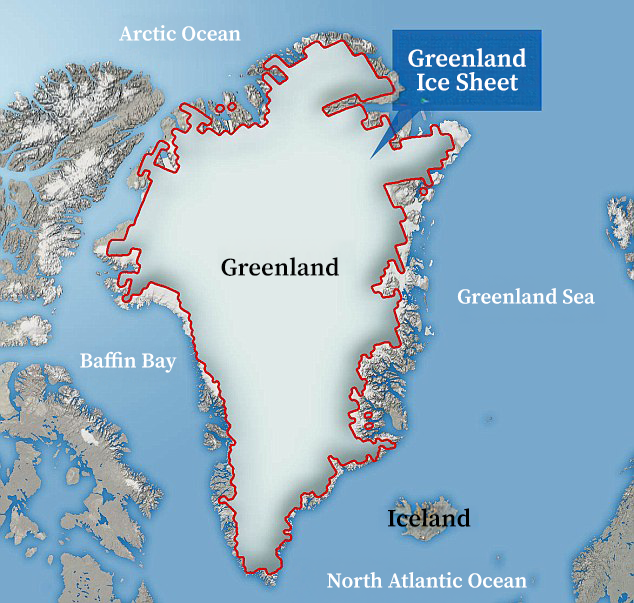
\includegraphics[width=0.5\linewidth]{images/greenland-ice-sheet.png}
        \caption{Ice Coverage Map of Greenland \citep{plummer2016greenland}}
        \label{fig:greenland-ice-map}
    \end{figure}
   Given these constraints, Greenland does not and cannot produce the majority of goods it consumes. It imports nearly all fuel, food, and manufactured items—more than 56\% of which are classified as consumer goods, followed by petroleum (24.5\%) and machinery (10.6\%). Its productive output is almost entirely concentrated in seafood, specifically shrimp and halibut. Shrimp and halibut alone accounted for over 56\% of its \$1.49 billion in exports, with seafood comprising more than 92\% overall. While over 49\% of Greenland’s exports were sent to Denmark, an even greater share—56\%—of its imports came from Denmark and the wider EU. This reciprocal trade relationship is supported by a longstanding agreement with the EU, which provides Greenland with preferential access to nearby European markets\footnote{As an Overseas Country and Territory (OCT) of the EU, Greenland benefits from tariff-free access for its fisheries exports under the EU-Greenland Fisheries Partnership Agreement \citep{oec2025}}. This institutional arrangement, supported by geographic proximity, has shaped Greenland’s trade profile  (Table~\ref{tab:greenland-trade}). With limited options for economic diversification, Greenland has leveraged its maritime access to the EU to develop a highly concentrated seafood export economy. 

\renewcommand{\arraystretch}{0.95}
\begin{table}[H]
\centering
\small
\begin{threeparttable}
\caption{Greenland’s Trade Profile \citep{oec2025}}
\label{tab:greenland-trade}
\begin{tabular}{@{}p{0.28\textwidth} p{0.28\textwidth} p{0.33\textwidth}@{}}
\toprule
\textbf{Major Exports} & \textbf{Major Imports} & \textbf{Top Trade Partners} \\
\midrule
Frozen Shrimps – 32.5\% \newline
Frozen Halibut – 24.3\% \newline
Prepared Shrimps – 17.3\% \newline
Frozen Fish Fillet – 7.0\% \newline
Frozen Cod – 4.6\% \newline
Crabs – 4.0\% \newline
Other Fish – 3.2\% \newline
Mackerel – 1.1\% \newline
Others – 4.9\% &

Consumer Goods – 56.2\% \newline
Refined Petroleum – 24.5\% \newline
Machinery – 10.6\% \newline
Aircraft – 8.9\% \newline
Cars, Trucks – 4.2\% \newline
Others – 5.4\% &

\textit{Top Export Destinations:} \newline
Denmark – 49.0\% \newline
China – 23.8\% \newline
United Kingdom – 5.8\% \newline
Japan – 5.2\% \newline
Chinese Taipei – 3.4\% \newline
\noindent\rule{\linewidth}{0.4pt} \newline
\textit{Top Import Origins:} \newline
Denmark – 56.1\% \newline
Sweden – 22.0\% \newline
France – 9.5\% \newline
Iceland – 2.8\% \newline
Canada – 2.7\%
\\
\bottomrule
\end{tabular}
\begin{tablenotes}
\footnotesize
Consumer goods have been aggregated into a single category due to the large number of individually small import items. While Greenland imports a wide range of consumer products—including clothing, furniture, tools, beverages, and household goods—each category comprises numerous low-value subcategories. 
\end{tablenotes}
\end{threeparttable}
\end{table}

    Clearly, Greenland’s specialization in seafood demonstrates the concept of comparative advantage. It takes advantage of the resources it has and maximizes export capacity despite severe structural constraints. Classical trade theory, as first formalized by David Ricardo\footnote{While Ricardo’s model emphasizes technological differences and allows for full specialization, other trade models—such as the Specific Factors and Heckscher–Ohlin models—generally predict partial specialization due to diminishing returns and reallocation across sectors. In practice, full specialization is rare. However, Greenland’s export profile—over 92\% concentrated in seafood—approximates this condition unusually well. Therefore, the Ricardian model is especially illustrative in this context.}, explains trade through differences in technology. A simple example could be a landlocked nation with efficient textile production but limited maritime infrastructure, and a coastal nation with advanced shipbuilding technology but low textile output. Rather than producing both goods themselves, each country gains more by specializing in what it can produce efficiently and trading for the rest. In Greenland’s case, this logic holds. With limited capacity to produce food, fuel, or industrial goods, it is effectively constrained to exploit its marine resources. As such, it exports seafood—the one sector in which it holds a comparative advantage—and imports nearly everything else.
    
    \subsection*{Too Expensive for Too Little: Is the U.S. After Greenlandic Seafood?}
    
    Given Greenland’s clear specialization in seafood, it might seem logical to assume that the United States would seek to deepen trade in this sector, especially because current exchange between the two remains minimal. That assumption, however, overlooks the fact that the U.S. seafood market is already well-served by more efficient suppliers with stronger existing ties. In 2024, the United States imported approximately \$30.4 billion worth of seafood, primarily from established partners such as Canada, China, Chile, Indonesia and India \citep{usda2025foodimports}. As shown in Figure~\ref{fig:seafood-imports}, these countries consistently dominate the U.S. import market. In contrast, Greenland makes up less than 0.1\% of total imports and barely registers in the U.S. seafood trade.
    
    \begin{figure}[H]
        \centering
        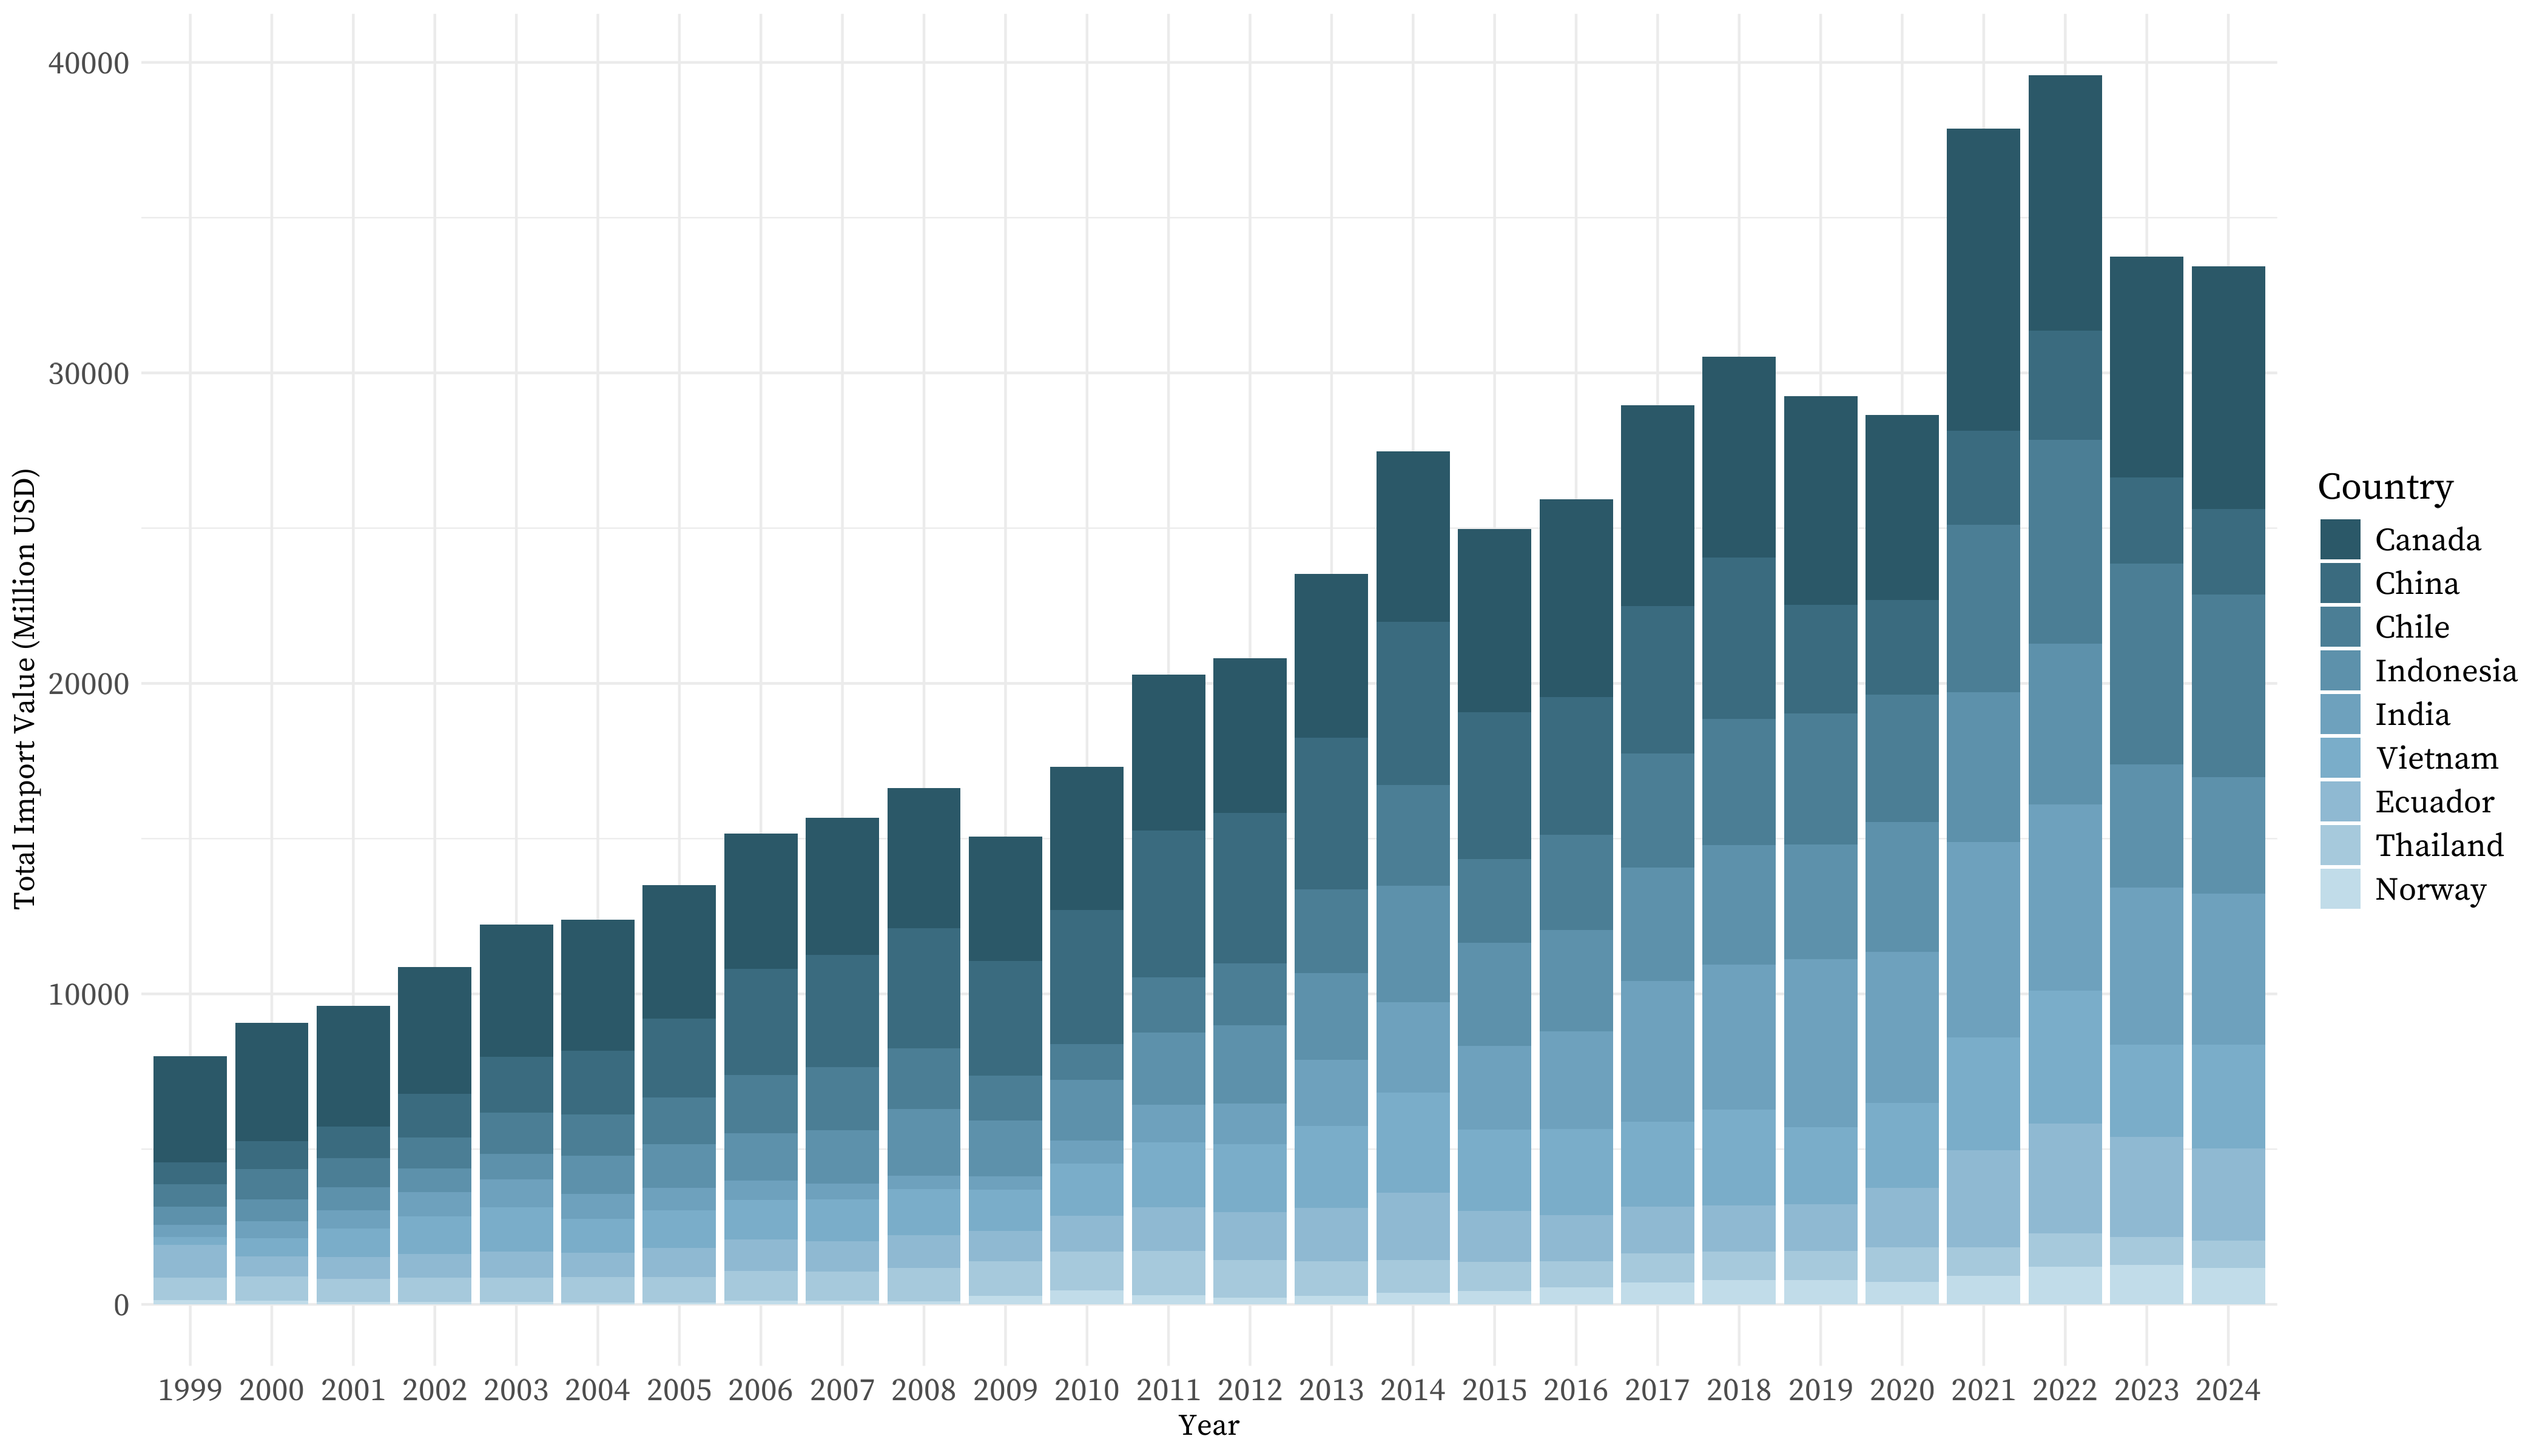
\includegraphics[width=0.90\linewidth]{images/seafood_imports_by_country.png}
        \caption{Annual U.S. Seafood Imports by Country, 1999–2024 \citep{usda2025foodimports}}
        \label{fig:seafood-imports}
    \end{figure}
    
    Furthermore, even though Nuuk is geographically closer to the U.S. eastern seaboard than to many European ports (Figure~\ref{fig:trade-routes}), shipping to the United States is significantly more expensive than existing routes to Europe. Estimates from \citet{royalarcticline2024freight} and maritime freight brokers suggest that refrigerated 20-foot container shipments from Nuuk to Denmark cost between \$1,800–\$3,800 depending on season and cargo. By contrast, shipping to the U.S. can run \$4,500–\$7,000 per container due to both distance and limited port infrastructure \citep{intlvanlines2024shipping}. These costs are further inflated by the Jones Act\footnote{The Jones Act has already raised shipping costs in other U.S.-controlled regions, such as Puerto Rico, where it has been widely criticized for inflating the price of imported goods and complicating emergency response efforts \citep{rivera2018hard}.}, which requires that any domestic leg of shipping within the United States be handled by U.S.-built, U.S.-flagged, and U.S.-crewed vessels. This effectively reduces port flexibility and increases transshipment costs for foreign exporters like Greenland. Meanwhile, as summarized in Table \ref{tab:seafood-shipping-costs}, the United States maintains far more cost-efficient seafood trade relationships with its top suppliers such as Canada, China, and Chile. 


    \begin{figure}[H]
        \centering
        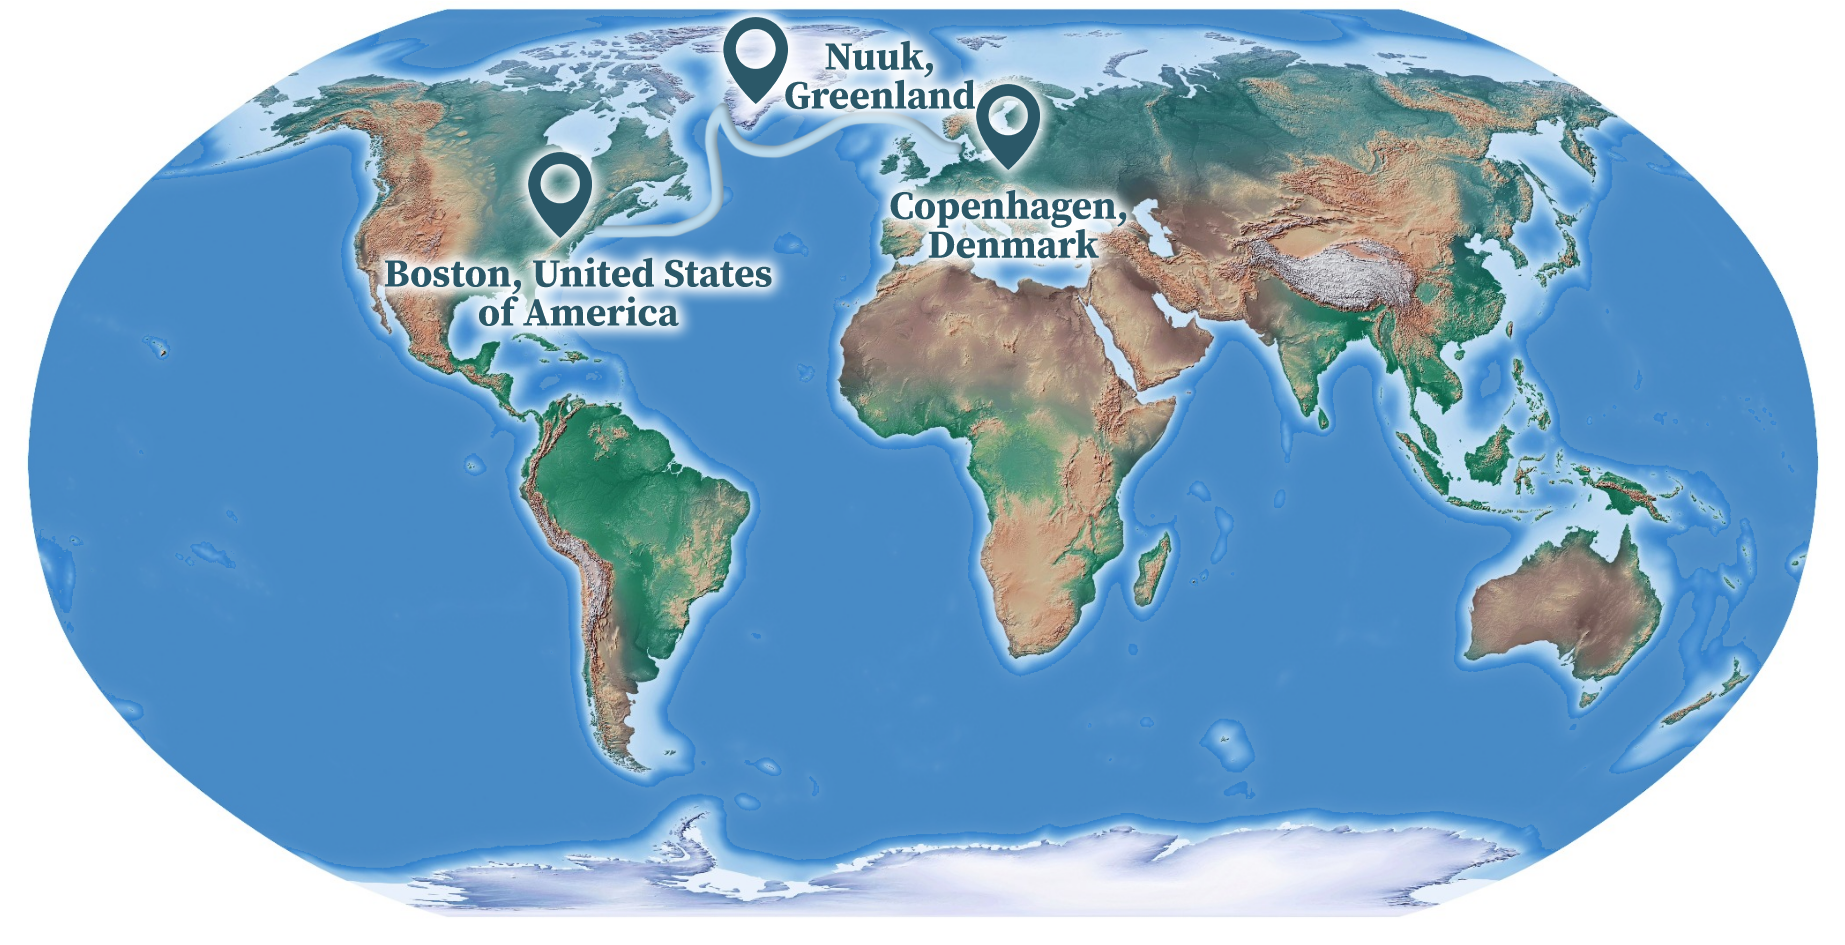
\includegraphics[width=.75\linewidth]{images/trade-routes.png}
        \caption{Approximate shipping routes from Nuuk, Greenland to Copenhagen, Denmark and Boston, United States. Distances and directions are approximate due to the absence of official point-to-point commercial routing data.}
        \label{fig:trade-routes}
    \end{figure}

    \renewcommand{\arraystretch}{0.95}
\begin{table}[H]
\centering
\small
\begin{threeparttable}
\caption{Estimated Shipping Costs of Top 5 Seafood Importers to the United States (2025) \citep{freightos2025canada, dantful2025china, icontainers2025chile, freightos2025indonesia, freightos2025india}}
\label{tab:seafood-shipping-costs}
\begin{tabular}{@{}l@{\hskip 6pt}r@{\hskip 6pt}r@{\hskip 6pt}p{5.2cm}@{}}
\toprule
\textbf{Country} & \textbf{20-ft Container (USD)} & \textbf{Air Freight per kg (USD)} & \textbf{Notes} \\
\midrule
Canada     & \$1,200–2,000 & \$2.00–4.00 & Proximity and established logistics reduce costs. \\
China      & \$2,500–4,200 & \$5.00–6.00 & Costs elevated by tariffs and high demand. \\
Chile      & \$1,800–3,800 & \$4.00–5.50 & Competitive rates supported by efficient ports and FTAs. \\
Indonesia  & \$2,000–3,500 & \$5.00–6.00 & Long transit times and weaker port infrastructure. \\
India      & \$2,700–4,000 & \$5.00–6.00 & Limited direct routes increase overall freight cost. \\
\bottomrule
\end{tabular}
\begin{tablenotes}
\footnotesize
\item Freight estimates may vary by carrier, port conditions, and seasonal factors. Air rates reflect average costs for refrigerated cargo. Shipping costs represent typical rates to major U.S. entry points such as Boston, New York, and Los Angeles, depending on the country of origin. Nonetheless, it is noteworthy that even the U.S. port geographically closest to Nuuk remains significantly more expensive than routes from more distant countries regardless of the destination port.
\end{tablenotes}
\end{threeparttable}
\end{table}

    Even if the United States were willing to overlook Greenland’s logistical challenges, it does little to reduce the opportunity cost. The U.S. seafood supply chain is already well-established with global producers, especially in Latin America and Southeast Asia, regions that collectively account for more than 60\% of total U.S. seafood imports. These trade relationships are reinforced by scale, logistical efficiency, and regulatory alignment that has developed over decades. Meanwhile, shifting procurement to Greenland would not only require a complete overhaul of the cold chain infrastructure, but also involve the navigation of misaligned inspection protocols\footnote{Greenland’s seafood exports are governed by EU sanitary and phytosanitary (SPS) protocols under the EU-Greenland Fisheries Partnership Agreement \citep{eufisheries2024greenland}. These include stringent rules on catch documentation, traceability, facility inspections, and hygiene requirements tailored to European market norms. In contrast, US imports are regulated by the US Department of Agriculture (USDA) and the Food and Drug Administration (FDA). The USDA oversees the labeling and classification of seafood for quality, while the FDA enforces safety standards under the Food Safety Modernization Act (FSMA), including hazard analysis (HACCP) plans and import certifications \citep{fda2025seafood}. Because these systems are not mutually recognized, Greenlandic seafood would require reprocessing or recertification to enter the U.S. market, which is an additional logistical and regulatory burden.} and limited shipping windows. For Washington, the strategic yield simply does not justify the cost.

    With all these inefficiencies, seafood alone does not sufficiently explain U.S. interest in Greenland. The sector is too small and economically marginal to support a major realignment in trade. The value of Greenland’s mineral deposits—as discussed earlier—offers a more plausible rationale, especially given its reserves of critical materials. As supply chains face mounting geopolitical pressures, these resources have become an increasingly relevant consideration.

    \subsection*{Security Over Savings: The Case for Trade Diversion}

    As established earlier, it is clear that seafood trade is not what the United States is pursuing with Greenland. This insistence runs counter to classical trade theory, which favors low-cost, efficiency-driven exchange. Yet, annexation cannot be evaluated solely through the lens of comparative advantage. Instead, it aligns more closely with the logic of trade diversion: the deliberate shift of sourcing away from a low-cost, high-risk supplier to a higher-cost but geopolitically stable one. 

    In recent years, American reliance on adversarial\footnote{In this context, 'adversarial' refers to countries that have a history of political, economic, or strategic tensions with the United States, such as China or Russia. These states may leverage economic dependencies to exert geopolitical pressure.} suppliers for critical minerals has been increasingly recognized as a form of strategic vulnerability. The concern became so pronounced that, during President Trump’s first term, it prompted an executive order,\footnote{The document is titled: Executive Order 13953, Addressing the Threat to the Domestic Supply Chain from Reliance on Critical Minerals from Foreign Adversaries and Supporting the Domestic Mining and Processing Industries.} which declared that such reliance constitutes “an unusual and extraordinary threat to the national security, foreign policy, and economy of the United States” \citep{executiveorder13953}.
    
    Nowhere is the risk more evident than in the rare earth supply chain, where U.S. dependence on a single geopolitical rival has already revealed the national consequences of such reliance. In 2020, China accounted for 74 percent of U.S. rare earth imports, and in 2023, it remained the dominant supplier of processed rare earth compounds and oxides. The United States also sources over 80 percent of certain rare earths from China, according to \citet{usgs_rare_earths}. In February 2025, Beijing imposed a new round of export bans on rare earth compounds, escalating its previous restrictions on gallium and germanium issued in 2023. These actions were widely interpreted as responses to Western technology controls and marked a clear use of economic leverage.
    
    The economic consequences are already being felt. \citet{anil2025antimony} estimate that the 2025 bans could raise global prices of certain rare earth elements by 250 to 500 percent in the short term. For the United States, this translates into billions of dollars in additional costs across industries that rely heavily on these inputs. These ripple effects have made it urgent for the United States to rewire its supply chains and reduce dependence on politically volatile sources.
    
   As a result, the United States has moved beyond short-term fixes and adopted a structural strategy focused on overhauling critical supply chains. The federal government now prioritizes long-term goals through targeted investment and strategic sourcing. In 2022, over \$800 million was allocated through the Defense Production Act to support domestic and allied sourcing of essential inputs \citep{garamone2022ndaa}. This momentum has only intensified. As of writing, the United States is actively pursuing expanded Compacts of Free Association (COFA)\footnote{The Compacts of Free Association (COFA) are agreements between the United States and several Pacific Island nations which grant the U.S. military basing rights and strategic access in exchange for financial aid, immigration privileges, and broad economic cooperation. Unlike free trade agreements (FTAs), which focus primarily on reducing tariffs and standardizing regulatory barriers, COFAs are rooted in geopolitical partnerships and can include provisions on resource extraction, environmental monitoring, and development funding. While the U.S. has several FTAs globally, it does not currently have a free trade agreement with Greenland, making any resource-related engagement more diplomatically and logistically complex.} with Pacific Island nations–and, increasingly, with resource-rich territories like Greenland–to secure privileged access to rare earth reserves and other critical minerals \citep{slattery2025association}. These agreements, while not tantamount to formal annexation, enable joint resource development under a stable legal framework.

    In parallel, U.S.-backed firms have begun exploring opportunities to excavate rare earth elements in Greenland and other politically aligned jurisdictions viewed as credible alternatives to Chinese supply chains \citep{volcovici2025greenland}. However, translating these ambitions into viable operations would likely confront overwhelming logistical, environmental, and geopolitical challenges. 
    
    Firstly, Greenland’s terrain is largely frozen year-round, and its port infrastructure remains underdeveloped relative to established global mining hubs. To reiterate, there are no railways, few interconnected roads, and limited deepwater access for industrial-scale shipping. Mining operations would require not only significant upfront capital but also sustained investment in seasonal logistics, workforce housing, ice-resistant equipment, and environmental permitting. 
    
    Simply building the infrastructure needed to make extraction viable—such as upgrading ports in Nuuk or constructing all-weather transport corridors—would take years and involve substantial political and financial risk. For instance, Greenland’s largest-ever infrastructure project, the expansion of airports in Nuuk and Ilulissat, carries an estimated cost of 3.7 billion Danish kroner (approximately \$495 million) and has faced concerns over potential cost overruns of up to a third beyond initial estimates \citep{asce2022airports, arctictoday2022overruns}. Additionally, the maintenance backlog for Greenlandic ports increased by 23\% from 2019 to 2020, demonstrating the ongoing challenges in sustaining and developing essential maritime infrastructure \citep{highnorth2021ports}.

     \begin{figure}[H]
        \centering
        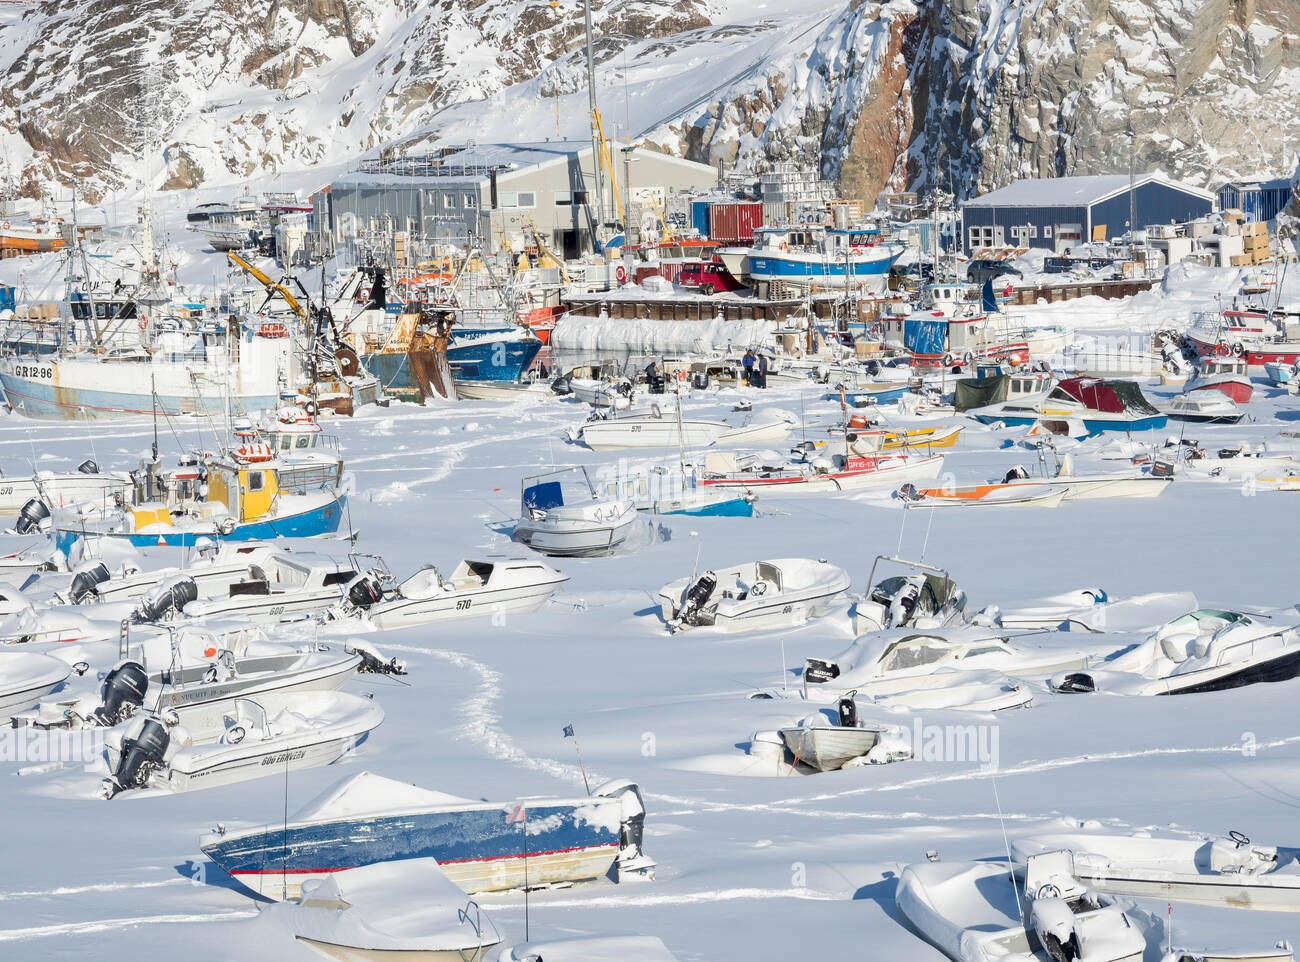
\includegraphics[width=0.58\linewidth]{images/frozen-harbor-with-fishing-boats-greenland-WAK1F6.jpg}
        \caption{Fishing boats frozen in the harbor of Nuuk, Greenland during winter \citep{alamy_wak1f6}}
        \label{fig:enter-label}
    \end{figure}

    Moreover, Greenland is a self-governing territory under the Kingdom of Denmark. Any unilateral U.S. effort to establish military or mining facilities without Denmark’s full consent could trigger diplomatic fallout with a key ally. Given Greenland’s close trade ties with the European Union through Denmark, aggressive U.S. investment to reduce Chinese influence could also strain relations with the EU\footnote{Following a call with President Donald Trump on January 15, 2025, Danish Prime Minister Mette Frederiksen confirmed renewed U.S. interest in acquiring Greenland and disclosed Washington’s threat to impose punitive sanctions on Denmark if it refused the transfer \citep{earle2025greenland}. In a meeting with Denmark’s parliamentary foreign policy committee, Frederiksen described the situation as “serious” and warned of potential fallout in Danish–U.S. economic cooperation and regional security \citep{reuters2025greenland}}. In particular, the European Union’s Anti-Coercion Instrument (ACI)—adopted in 2023 to counter economic pressure from non-EU countries—offers a legal mechanism for retaliation. Originally invoked in response to China’s trade restrictions on Lithuania over Taiwan, the ACI has since been cited in discussions of U.S. industrial policy and could be activated if Washington’s actions are perceived as coercive or destabilizing \citep{wu2023aci, europarl2023aci}. 

     Even in the best-case scenario—where logistical barriers are resolved and European partners remain cooperative—projections indicate that mining and refining operations in Greenland would still require 5–10 years to reach export scale \citep{greenland2025strategy}. This delay limits Greenland’s ability to serve as a near-term alternative to China’s rare earth dominance. On the other hand, yielding to China in targeted segments of the trade war—such as rare earth processing—may offer lower short-term costs. Unlike Greenland, China already possesses a mature and vertically integrated ecosystem for extraction, refining, and export, built over decades of state-backed investment \citep{holslag2022controlling}. In contrast, even if mining in Greenland proves successful, its minerals would still need to be shipped thousands of miles and refined elsewhere. As discussed earlier, these logistics are significantly more expensive than comparable routes from suppliers across Asia. 
     
     Nonetheless, the price of dependence–economic coercion, geopolitical vulnerability, and supply chain instability–has prompted the United States to consider costlier, less efficient sources as part of a major strategic reorientation. This is trade diversion in practice: a deliberate shift away from the most efficient supplier toward what the U.S. perceives as a more politically cooperative partner, despite higher costs and no guarantee of sustained strategic partnership. Still, the government’s willingness to absorb these costs and confront operational risks reflects a shift in priorities from short-term economic efficiency to long-term supply security, even amid heightened uncertainty.

    \subsection*{From Theory to Territory: Trade in the Age of Control}

    The Greenland case invites a reconsideration of how international trade theory accounts for a nation's behavior under conditions of geopolitical uncertainty. As with all economic models, simplification is a necessary feature–not a flaw\footnote{All economic models abstract away from certain real-world complexities to isolate specific mechanisms and generate testable predictions. As Joan Robinson once noted, "A model which took account of all the variegation of reality would be no more use than a map at the scale of one to one." The value of a model lies not in its completeness, but in its ability to clarify relationships under defined conditions.}. Within these frameworks, Greenland’s seafood export orientation toward the European Union is a textbook example of comparative advantage. However, such models offer limited explanatory power in contexts where trade is driven less by technological differences and more by geopolitical strategies. These developments are not anomalies in need of dismissal, but signals that a parallel logic increasingly governs international exchange. Furthermore, this is also not to suggest that trade theory is obsolete. It definitely remains essential for understanding cost-efficiency and patterns of specialization. However, when states prioritize supply geopolitical security over economic efficiency, they adopt a different logic. This is the concept of trade diversion, where sourcing shifts from the most efficient supplier to one that is considered more secure, even at a higher cost. 
    
    An additional consideration is whether strategic diversion would ultimately enhance or diminish overall welfare. The answer depends on the trade-off between the potential gains from sourcing minerals in Greenland and the losses associated with reducing imports from more efficient suppliers—namely, China. In Greenland’s case, the net effect remains uncertain, particularly as developments continue to unfold beyond the scope of this paper. Nonetheless, several factors suggest that welfare losses are likely to outweigh any potential gains. These include high start-up costs, severe logistical barriers, legal constraints under the Jones Act, and the risk of retaliatory measures from the European Union if U.S. actions are perceived as coercive. Even if those challenges were overcome, annexation would likely sever Greenland’s preferential access to the EU market and terminate its fiscal grant from Denmark—which currently covers approximately half of its government budget and would likely become a U.S. obligation. Taken together, these obstacles cast serious doubt on the long-term viability of strategic diversion toward Greenland.
    
    As the United States weighs whether the “grass is truly greener” on Greenland’s side—whether through the lens of classical trade theory or geopolitical ambitions rooted in trade diversion—it must account for the significant opportunity costs involved. Under Ricardo’s framework, Greenland’s comparative advantage lies in seafood—a sector with limited relevance to U.S. strategic interests. Pursuing its mineral reserves instead means abandoning efficiency, incurring high start-up costs, and redirecting trade away from relatively lower-cost suppliers like China. Meanwhile, trade diversion accepts such inefficiencies in favor of security and insulation. The answer to whether the grass is truly greener, then, depends on which logic the United States chooses to follow. Under Ricardo, Greenland offers little gain. Under diversion, it becomes a calculated risk—but one with substantial costs.
    
\printbibliography
	
\end{document}